\chapter{PENGUJIAN DAN EVALUASI}

\section{Lingkungan Uji Coba}
	Lingkungan pengujian menggunakan komponen-komponen yang terdiri dari: satu \textit{server load balancer}, satu \textit{server master host}, satu \textit{server controller}, satu \textit{server docker registry}, dan enam komputer penguji. Semua \textit{server} menggunakan Virtual Private Server dari DigitalOcean. Lalu, untuk komputer penguji menggunakan lima buah desktop dan satu buah VPS sebagai \textit{docker} klien yang digunakan untuk membuat \textit{docker image}. Pengujian dilakukan di Laboratoriom Pemrograman Jurusan Teknik Informatika ITS. \\
    \indent Spesifikasi untuk setiap komponen yang digunakan ditunjukkan pada Tabel \ref{spesifikasikomponen}.
    \begin{longtable}{|p{0.05\textwidth}|p{0.18\textwidth}|p{0.33\textwidth}|p{0.33\textwidth}|}					\caption{Spesifikasi Komponen} \label{spesifikasikomponen} \\
        \hline
        \textbf{No} & \textbf{Komponen} & \textbf{Perangkat Keras} & \textbf{Perangkat Lunak} \\ \hline
        \endfirsthead
        \caption[]{Spesifikasi Komponen} \\
        \hline
        \textbf{No} & \textbf{Komponen} & \textbf{Perangkat Keras} & \textbf{Perangkat Lunak} \\ \hline
        \endhead
        \endfoot
        \endlastfoot

    	1 & Load balancer & 2 core processor, 4GB RAM, 20GB SSD & Ubuntu 14.04.5 LTS, HAProxy, Python 2.7 \\ \hline
        2 & Master host & 8 core processor, 16GB RAM, 20GB SSD & Ubuntu 14.04.5 LTS, Docker 17.03.0-ce, Python 2.7 \\ \hline
        3 & Controller & 2 core processor, 4GB RAM, 20GB SSD & Ubuntu 14.04.5 LTS, Redis, MySQL, Python 2.7 \\ \hline
        4 & Docker registry & 1 core processor, 512MB RAM, 20GB SSD & Ubuntu 14.04.5 LTS, Docker 17.03.0-ce, Python 2.7 \\ \hline
        5 & Komputer penguji & Processor Core2Duo E7300, 2GB RAM & Windows 8, JMeter 3.2 \\ \hline
        6 & Docker klien & 1 core processor, 1GB RAM, 20GB SSD & Ubuntu 16.04 LTS, Docker 17.03.0-ce \\ \hline
    \end{longtable}
    
    \indent Untuk akses ke masing-masing komponen, digunakan IP publik yang disediakan untuk masing-masing komponen tersebut. Selain menggunakan IP, ada sebagian \textit{server} yang bisa diakses melalui domain. Detailnya ditunjukkan pada Tabel \ref{ipdomainserver}.
    			\begin{longtable}{|p{0.05\textwidth}|p{0.33\textwidth}|p{0.44\textwidth}|}					\caption{IP dan Domain Server} \label{ipdomainserver} \\
					\hline
					\textbf{No} & \textbf{Server} & \textbf{IP dan Domain} \\ \hline
					\endfirsthead
					\caption[]{IP dan Domain Server} \\
					\hline
					\textbf{No} & \textbf{Server} & \textbf{IP dan Domain} \\ \hline
					\endhead
					\endfoot
					\endlastfoot
					
                    1 & Load balancer & 128.199.160.188 \\ \hline
                    2 & Master host & 128.199.182.29 \\ \hline
                    3 & Controller & 128.199.250.137 http://controller.nota-no.life \\ \hline
                    4 & Docker registry & 139.59.97.244 https://registry.nota-no.life \\ \hline
				\end{longtable}
    
\section{Skenario Uji Coba} \label{skenarioujicoba}
	Uji coba akan dilakukan untuk mengetahui keberhasilan sistem yang telah dibangun. Skenario pengujian dibedakan menjadi 2 bagian, yaitu:
    \begin{itemize}
    \item \textbf{Uji Fungsionalitas} \\
    	Pengujian ini didasrkan pada fungsionalitas yang disajikan sistem.
    \item \textbf{Uji Performa} \\
    	Pengujian ini untuk menguji ketahanan sistem terhadap sejumlah permintaan ke aplikasi secara bersamaan. Pengujian dilakukan dengan melakukan \textit{benchmark} pada sistem.
    \end{itemize}
    
    \subsection{Skenario Uji Coba Fungsionalitas}
    	Uji fungsionalitas dibagi menjadi 2, yaitu uji mengelola aplikasi berbasis \textit{docker} dan uji fungsionalitas menu aplikasi Dasbor.
        
        \subsubsection{Uji Mengelola Aplikasi Berbasis Docker} \label{ujimengelolaaplikasiberbasisdocker}
        	Pengujian ini dilakukan untuk mengetahui apakah sistem sudah bisa menyimpan dan mengelola data \textit{docker image} dari aplikasi yang dimasukkan oleh pengembang. Pengujian menggunakan VPS yang berperan sebagai \textit{docker} klien. Pengujian dilakukan dengan memasukkan data \textit{docker image} ke \textit{server docker registry} yang sudah disediakan. Dengan menggunakan sebuah komputer lain yang digunakan untuk membuat aplikasi web berbasis \textit{docker}, dari sana aplikasi tersebut akan ditaruh ke \textit{server docker registry}. \\
            \indent Alamat dari Docker \textit{registry} yang digunakan adalah \texttt{https://registry.nota-no.life}. Setelah berhasil melakukan login pada \textit{server docker registry}, selanjutnya adalah memasukkan \textit{image} baru tersebut. \textit{Image} yang dibuat adalah sebuah aplikasi web berbasis PHP 7 dengan \textit{web server} Apache. Aplikasi web tersebut menyediakan sebuah halaman yang berisi sebuah teks yang dibuat melalui pemanggilan fungsi PHP. \\
            \indent Pertama kali \textit{image} tersebut dimasukkan ke \textit{server docker registry}, kemudian data dari \textit{image} tersebut akan disimpan di \textit{server controller}. Setelah data tersimpan, selanjutnya adalah menjalankan aplikasi melalui dasbor yang disediakan. Sebelum menjalankan aplikasi, terlebih dahulu mengatur \textit{port} dari aplikasi yang akan berjalan. Setelah mengatur \textit{port} dengan benar, selanjutnya adalah menjalankan aplikasinya. Jika aplikasi berhasil dijalankan, maka aplikasi dapat diakses melalui domain yang disediakan. \\
            \indent Setelah aplikasi berjalan, selanjutnya adalah memperbarui aplikasi dengan mengganti teks yang ditampilkan. Untuk itu, pada komputer yang digunakan untuk membuat \textit{image} sebelumnya, maka dibuatkan image baru dari aplikasi dengan versi terbaru. Image versi terbaru ini kemudian di \textit{push} ke \textit{docker registry}. Setelah selesai melakukan \textit{push}, harapannya aplikasi yang sebelumnya sudah berjalan, akan diperbarui secara otomatis oleh sistem. \\
            \indent Terakhir, pengujian yang dilakukan adalah menghentikan aplikasi yang sudah berjalan. Fungsi untuk menghentikan aplikasi yang sedang berjalan ini terdapat pada dasbor. Jika proses ini berhasil, maka domain yang sebelumnya digunakan untuk mengakses aplikasi akan hilang dan pengguna tidak bisa lagi melakukan akses terhadap aplikasi. \\
            \indent Daftar uji fungsionalitas menambahkan dan memperbarui aplikasi dijelaskan pada Tabel \ref{ujiaplikasi}.
            \begin{longtable}{|p{0.05\textwidth}|p{0.38\textwidth}|p{0.39\textwidth}|}					\caption{Skenario Uji Mengelola Aplikasi Berbasis Docker} \label{ujiaplikasi} \\
					\hline
					\textbf{No} & \textbf{Uji Coba} & \textbf{Hasil Harapan} \\ \hline
					\endfirsthead
					\caption[]{Skenario Uji Mengelola Aplikasi Berbasis Docker} \\
					\hline
					\textbf{No} & \textbf{Uji Coba} & \textbf{Hasil Harapan} \\ \hline
					\endhead
					\endfoot
					\endlastfoot
					
                    1 & Pengguna melakukan \textit{login} ke \textit{server docker registry} & Pengguna berhasil melakukan \textit{login} dengan menggunakan \textit{username} dan \textit{password} yang sudah ditentukan. \\ \hline
                    2 & Pengguna menambahkan \textit{image} baru dari sebuah aplikasi ke \textit{server docker registry}. & Pengguna berhasil menambahkan \textit{image} baru dan data tersimpan pada \textit{server controller}. \\ \hline
                    3 & Pengguna bisa mengatur \textit{port} dari aplikasi menggunakan dasbor yang disediakan & Data \textit{port} dari aplikasi yang tersimpan bisa diganti sesuai dengan kebutuhan pengguna. \\ \hline
                    4 & Pengguna bisa menjalankan aplikasi melalui fitur yang ada pada dasbor & Aplikasi berhasil berjalan dan pengguna mendapatkan domain yang digunakan untuk mengakses aplikasi. \\ \hline
					5 & Pengguna memperbarui aplikasi yang sedang berjalan dengan melakukan \textit{push} ke \textit{server docker registry}. & Aplikasi yang sedang berjalan akan diperbarui secara otomatis tanpa perlu perintah dari pengguna. \\ \hline
                    6 & Penggua menghentikan aplikasi yang sedang berjalan. & Aplikasi berhasil dihentikan dan pengguna tidak bisa lagi melakukan akses aplikasi. \\ \hline
				\end{longtable}
            
        \subsubsection{Uji Fungsionalitas Menu Aplikasi Dasbor}
        	Aplikasi Dasbor digunakan untuk mengelola dan memantau aplikasi. Aplikasi Dasbor terdiri dari 4 bagian utama, yaitu halaman beranda, informasi aplikasi, informasi \textit{container}, dan metrik dari aplikasi. Rancangan pengujian dan hasil yang diharapkan ditunjukkan dengan Tabel \ref{skenarioUjiDasboard}.
            
            \begin{longtable}{|p{0.05\textwidth}|p{0.20\textwidth}|p{0.30\textwidth}|p{0.27\textwidth}|}
						\caption{Skenario Uji Fungsionalitas Aplikasi Dasbor} \label{skenarioUjiDasboard} \\
						\hline
						\textbf{No} & \textbf{Menu} & \textbf{Uji Coba} & \textbf{Hasil Harapan} \\ \hline
						\endfirsthead
						\caption[]{Skenario Uji Fungsionalitas Aplikasi Dasbor}  \\
						\hline
						\textbf{No} & \textbf{Menu} & \textbf{Uji Coba} & \textbf{Hasil Harapan} \\ \hline
						\endhead
						\endfoot
						\endlastfoot
						1 & Kelola aplikasi & Menambahkan aplikasi baru atau memperbarui aplikasi & Dasbor dapat menampilkan daftar aplikasi terbaru yang dimasukkan atau diperbarui oleh pengembang. \\ \cline{3-4}
                        && Menjalankan aplikasi yang sudah masuk ke dalam sistem & Aplikasi dapat berjalan dan pengguna mendapatkan domain untuk mengakses aplikasi. \\ \cline{3-4}
                        && Menghentikan aplikasi yang sedang berjalan & Aplikasi yang sedang berjalan dapat dihentikan dan pengguna tidak bisa lagi melakukan akses terhadap aplikasi. \\ \cline{3-4}
                        && Mengganti \textit{port} aplikasi agar dapat berjalan dengan baik & Pengguna dapat mengganti \textit{port} aplikasi agar aplikasi dapat berjalan dengan benar. \\ \hline
						2 & Lihat informasi aplikasi & Memilih salah satu aplikasi yang ada  & Pengguna dapat melihat infromasi secara lengkap tentang aplikasi. \\ \hline
                        3 & Lihat informasi \textit{container} & Memilih salah satu aplikasi yang ada  & Pengguna dapat melihat infromasi secara lengkap tentang \textit{container} yang sedang berjalan untuk aplikasi tersebut. \\ \hline
                        4 & Lihat metrik aplikasi & Memilih salah satu aplikasi yang ada  & Pengguna dapat melihat grafik penggunaan CPU dan \textit{memory} dari aplikasi . \\ \hline
					\end{longtable}
        
    \subsection{Skenario Uji Coba Performa}
    	Uji performa dilakukan dengan menggunakan lima buah desktop untuk melakukan akses secara bersamaan ke aplikasi menggunakan aplikasi JMeter. Desktop akan mencoba mengaskses halaman dari aplikasi web yang sudah berjalan, dengan domain aplikasi.nota-no.life. Halaman yang akan diakses berisi sebuah teks yang dihasilkan dari pemanggilan fungsi PHP. \\
        \indent Percobaan dilakukan dengan lima skenario jumlah \textit{concurrent user} yang berbeda, yaitu sebanyak 800, 1600, 2400, 3200, dan 4000 pengguna dalam rentang waktu inisialisasi $\pm$ 15 detik. Waktu tersebut menunjukkan masing-masing pengguna akan mengirimkan request selama $\pm$ 15 detik, namun tidak termasuk waktu menunggu balasan dari \textit{server}, yang artinya keseluruhan permintaan tersebut akan lebih dari waktu tersebut dan bergantung pada kemampuan \textit{server} untuk memberikan respon. Pengujian \textit{request} ini bertujuan untuk mengukur kemampuan dari \textit{proactive model}. Untuk masing-masingnya, dicoba sebanyak empat perhitungan \textit{proactive model} yang berbeda menggunakan ARIMA yang berbeda, yaitu ARIMA(1,1,0), ARIMA(2,1,0), ARIMA(3,1,0), ARIMA(4,1,0). \textit{Proactive model} sendiri berguna untuk mengetahui jumlah \textit{request} kedepannya agar sistem bisa menyediakan sumber daya berdasarkan predeksi tersebut. \\
        \indent Selain itu, untuk memperkirakan sumber daya yang dibutuhkan sistem kedepannya, digunakan \textit{reactive model}. \textit{Model} tersebut akan menghitung jumlah \textit{container} yang sumber daya CPU dan \textit{memory}-nya sudah melebihi batas yang ditentukan. Sistem akan membentuk \textit{container} baru berdasarkan perhitungan \textit{reactive model} tersebut jika ada \textit{container} yang penggunaannya sudah melebihi batas atas dan mengurangi \textit{container} jika ada \textit{container} yang tidak digunakan. Percobaan akan dilakukan sebanyak enam kali dan berikutnya akan dijelaskan data apa yang diuji untuk masing-masingnya. \\
        \indent
    	\subsubsection{Uji Performa Kecepatan Menangani \textit{Request}}
        	Pengujian dilakukan dengan mengukur jumlah waktu yang diperlukan untuk menyelesaikan \textit{request} yang dilakukan oleh komputer penguji. Waktu yang diukur adalah perbedaan jarak antara \textit{request} pertama dan yang terakhir dilakukan oleh klien yang mendapatkan balasan dari \textit{server}.
        \subsubsection{Uji Performa Penggunaan CPU}
        	Pengujian dilakukan dengan menghitung penggunaan CPU yang terjadi pada \textit{server master host}. Penggunaan CPU di sini adalah penggunaan dari \textit{container} aplikasi yang sedang berjalan. Perhitungan dilakukan dengan mengambil nilai rata-rata penggunaan CPU dari masing-masing \textit{container} selama proses pengujian dilakukan. Nilai yang didaptkan berupa total persen penggunaan CPU oleh \textit{container} dibandingkan dengan keseluruhan kemampuan CPU.
        \subsubsection{Uji Performa Penggunaan \textit{Memory}}
        	Pengujian dilakukan dengan menghitung penggunaan \textit{memory} yang terjadi pada \textit{server master host}. Penggunaan \textit{memory} di sini adalah penggunaan dari \textit{container} aplikasi yang sedang berjalan. Perhitungan dilakukan dengan mengambil nilai rata-rata pengguanaan \textit{memory} dari masing-masing aplikasi selama proses pengujian dilakukan.
        \subsubsection{Uji Performa Keberhasilan \textit{Request}}
        	Pengujian dilakukan dengan menghitung jumlah \textit{request} yang gagal dilakukan selama skenario dijalankan. Dari semua jumlah \textit{request} yang dikirimkan selama pengujian, akan didapatkan persen \textit{request} yang gagal dilakukan.
    
\section{Hasil Uji Coba dan Evaluasi}
	Berikut dijelaskan hasil uji coba dan evaluasi berdasarkan skenario yang telah dijelaskan pada subbab \ref{skenarioujicoba}.
    
	\subsection{Uji Fungsionalitas}
    	Berikut dijelaskan hasil pengujian fungsionalitas pada sistem yang dibangun.
        
        \subsubsection{Uji Mengelola Aplikasi Berbasis Docker}
    	Pengujian dilakukan sesuai dengan skenario yang dijelaskan pada subbab \ref{ujimengelolaaplikasiberbasisdocker} dan pada Tabel \ref{ujiaplikasi}. Hasil pengujian seperti tertera pada Tabel \ref{hasilujicobaaplikasi}.
        
        \begin{longtable}{|p{0.05\textwidth}|p{0.55\textwidth}|p{0.22\textwidth}|}					\caption{Hasil Uji Coba Mengelola Aplikasi Berbasis Docker} \label{hasilujicobaaplikasi} \\
					\hline
					\textbf{No} & \textbf{Uji Coba} & \textbf{Hasil} \\ \hline
					\endfirsthead
					\caption[]{Hasil Uji Coba Mengelola Aplikasi Berbasis Docker} \\
					\hline
					\textbf{No} & \textbf{Uji Coba} & \textbf{Hasil} \\ \hline
					\endhead
					\endfoot
					\endlastfoot
					
                    1 & Pengguna melakukan \textit{login} ke \textit{server docker registry} & OK. \\ \hline
                    2 & Pengguna menambahkan \textit{image} baru dari sebuah aplikasi ke \textit{server docker registry}. & OK. \\ \hline
                    3 & Pengguna bisa mengatur \textit{port} dari aplikasi menggunakan dasbor yang disediakan & OK. \\ \hline
                    4 & Pengguna bisa menjalankan aplikasi melalui fitur yang ada pada dasbor. & OK. \\ \hline
					5 & Pengguna memperbarui aplikasi yang sedang berjalan dengan melakukan \textit{push} ke \textit{server docker registry}. & OK. \\ \hline
                    6 & Penggua menghentikan aplikasi yang sedang berjalan. & OK. \\ \hline
				\end{longtable}
    		Sesuai dengan skenario uji coba  yang diberikan pada Tabel \ref{ujiaplikasi}, hasil uji coba menunjukkan semua skenario berhasil ditangani.
        
    	\subsubsection{Uji Fungsionalitas Menu Aplikasi Dasbor}
        	Sesuai dengan skenario pengujian yang dilakukan pada aplikasi dasbor. Pengujian dilakukan dengan menguji setiap menu pada aplikasi dasbor. Hasil uji coba dapat dilihat pada Table \ref{hasilUjiDasboard}. Semua skenario yang direncanakan berhasil ditangani.
        		\begin{longtable}{|p{0.05\textwidth}|p{0.20\textwidth}|p{0.30\textwidth}|p{0.27\textwidth}|}
						\caption{Hasil Uji Fungsionalitas Aplikasi Dasbor} \label{hasilUjiDasboard} \\
						\hline
						\textbf{No} & \textbf{Menu} & \textbf{Uji Coba} & \textbf{Hasil} \\ \hline
						\endfirsthead
						\caption[]{Hasil Uji Fungsionalitas Aplikasi Dasbor}  \\
						\hline
						\textbf{No} & \textbf{Menu} & \textbf{Uji Coba} & \textbf{Hasil} \\ \hline
						\endhead
						\endfoot
						\endlastfoot
						1 & Kelola aplikasi & Menambahkan aplikasi baru atau memperbarui aplikasi & Dasbor berhasil menampilkan daftar aplikasi terbaru yang dimasukkan atau diperbarui oleh pengembang. \\ \cline{3-4}
                        && Menjalankan aplikasi yang sudah masuk ke dalam sistem & Aplikasi berhasil berjalan dan pengguna mendapatkan domain untuk mengakses aplikasi. \\ \cline{3-4}
                        && Menghentikan aplikasi yang sedang berjalan & Aplikasi yang sedang berjalan berhasil dihentikan dan pengguna tidak bisa lagi melakukan akses terhadap aplikasi. \\ \cline{3-4}
                        && Mengganti \textit{port} aplikasi agar dapat berjalan dengan baik & Pengguna berhasil mengganti \textit{port} aplikasi agar aplikasi dapat berjalan dengan benar. \\ \hline
						2 & Lihat informasi aplikasi & Memilih salah satu aplikasi yang ada  & Pengguna berhasil melihat infromasi secara lengkap tentang aplikasi. \\ \hline
                        3 & Lihat informasi \textit{container} & Memilih salah satu aplikasi yang ada  & Pengguna berhasil melihat infromasi secara lengkap tentang \textit{container} yang sedang berjalan untuk aplikasi tersebut. \\ \hline
                        4 & Lihat metrik aplikasi & Memilih salah satu aplikasi yang ada  & Pengguna berhasil melihat grafik penggunaan CPU dan \textit{memory} dari aplikasi . \\ \hline
					\end{longtable}
    \pagebreak
    \subsection{Hasil Uji Performa}
    	Seperti yang sudah dijelaskan pada subbab \ref{skenarioujicoba} pengujian performa dilakukan dengan melakukan akses ke aplikasi dengan sejumlah pengguna secara bersama-sama. Pengujian dilaukan dengan memberikan \textit{request} secara berkelanjutan dengan jumlah pengguna terdiri dari lima bagian, yaitu 800, 1600, 2400, 3200, dan 4000 pengguna. Untuk jumlah \textit{request} yang dihasilkan dari masing-masing pengguna selama rentang waktu request $\pm$ 15 detik dapat dilihat pada Tabel \ref{trequest}. Jumlah tersebut akan diolah oleh \textit{reactive model}. Lalu jumlah penggunaan CPU dan memory selama menangani \textit{request} tersebut akan digunakan oleh \textit{proactive model} untuk menambahkan atau mengurangi \textit{container} yang ada.
        \begin{longtable}{|p{0.33\textwidth}|p{0.35\textwidth}|}
        \caption{Jumlah \textit{Request} ke Aplikasi} \label{trequest} \\
            \hline
            \textbf{\textit{Concurrent Users}} & \textbf{Jumlah \textit{Request}} \\ \hline
            \endfirsthead
            \caption[]{Jumlah \textit{Request} ke Aplikasi} \\
            \hline
            \textbf{\textit{Concurrent Users}} & \textbf{Jumlah \textit{Request}} \\ \hline
            \endhead
            \endfoot
            \endlastfoot
            
            800 & $\pm$ 16.925 \\ \hline
            1.600 & $\pm$ 26.650 \\ \hline
            2.400 & $\pm$ 34.943 \\ \hline
            3.200 & $\pm$ 50.092 \\ \hline
            4.000 & $\pm$ 57.750 \\ \hline
					
		\end{longtable}
        
        Pada Tabel \ref{tjumlahcontainer} dapat dilihat jumlah \textit{container} yang terbentuk selama proses \textit{request} dari \textit{user} yang dilakukan selama enam kali. Nilai yang ditampilkan berupa nilai rata-rata selama percobaan dibulatkan ke atas. Sistem dapat menyediakan \textit{container} sesuai dengan jumlah \textit{request} yang diberikan, semakin banyak \textit{request} yang dilakukan, maka \textit{container} yang disediakan akan semakin banyak. Nilai \textit{container} tersebut didapatkan dari perhitungan \textit{proactive model}. Selain melihat jumlah \textit{request}, penentuan \textit{container} yang dibentuk juga dari jumlah sumber daya yang digunakan \textit{container} berdasarkan perhitungan menggunakan \textit{reactive model}. Pada Gambar \ref{gjumlahcontainer} dapat dilihat grafik dari jumlah \textit{container} yang terbentuk berdasarkan jumlah \textit{request} yang dilakukan.
        
        \begin{longtable}{|p{0.25\textwidth}|p{0.20\textwidth}|p{0.20\textwidth}|}
        \caption{Jumlah \textit{Container}} \label{tjumlahcontainer} \\
            \hline
            \textbf{\textit{Concurrent Users}} & \textbf{Maksimal \textit{Container}} &  \textbf{Rata-rata \textit{Container}} \\ \hline
            \endfirsthead
            \caption[]{Jumlah \textit{Container}} \\
            \hline
            \textbf{\textit{Concurrent Users}} & \textbf{Maksimal \textit{Container}} &  \textbf{Rata-rata \textit{Container}} \\ \hline
            \endhead
            \endfoot
            \endlastfoot
            
            800 & 6 & 2 \\ \hline
            1.600 & 8 & 3 \\ \hline
            2.400 & 14 & 6 \\ \hline
            3.200 & 18 & 7 \\ \hline
            4.000 & 30 & 11 \\ \hline
					
		\end{longtable}
        
        \begin{figure}[H]
				\centering
				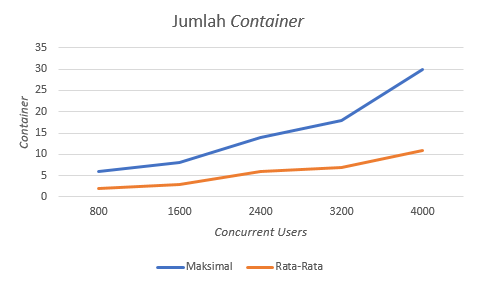
\includegraphics[width=8.7cm,height=4.7cm]{Images/C-5/jumlahcontainer.png}
				\caption{Grafik Jumlah \textit{Container}}
				\label{gjumlahcontainer}
			\end{figure}
        
    	\subsubsection{Kecepatan Menangani \textit{Request}}
        	Dari hasil uji coba kecepatan menangani \textit{request}, dapat dilihat pada Table \ref{kecepatanrequest} dalam satuan detik bahwa semakin banyak \textit{concurrent users}, semakin lama pula waktu yang diperlukan untuk menyeselaikannya. Request paling cepat ditangani dengan menggunakan prediksi ARIMA(4,1,0) dan paling lambat menggunakan ARIMA(1,1,0). Hal tersebut terjadi karena kurang bagusnya hasil prediksi yang dihasilkan oleh ARIMA(1,1,0) yang mana kadang hasil prediksinya terlalu rendah atau terlalu tinggi.
            Dari hasil percobaan tersebut, dapat dilihat bahwa hampir semua \textit{request} dapat ditangani di bawah satu menit. Lalu grafik hasil uji coba perhitungan kecepatan menangani \textit{request} ditunjukkan pada Gambar \ref{grunningtime}.
            \begin{longtable}{|p{0.22\textwidth}|p{0.10\textwidth}|p{0.10\textwidth}|p{0.10\textwidth}|p{0.10\textwidth}|p{0.10\textwidth}|}
        \caption{Kecepatan Menangani \textit{Request}} \label{kecepatanrequest} \\
            \hline
            & \textbf{800} & \textbf{1600} & \textbf{2400} & \textbf{3200} & \textbf{4000} \\ \hline
            \endfirsthead
            \caption[]{Kecepatan Menangani \textit{Request}} \\
            \hline
            & \textbf{800} & \textbf{1600} & \textbf{2400} & \textbf{3200} & \textbf{4000} \\ \hline
            \endhead
            \endfoot
            \endlastfoot
			
          	ARIMA(1,1,0) & 34.167 & 43.286 & 48.143 & 63.857 & 62.286 \\ \hline
            ARIMA(2,1,0) & 27.429 & 38.571 & 44.143 & 42.143 & 57.857 \\ \hline
            ARIMA(3,1,0) & 32.429 & 36.000 & 38.429 & 41.571 & 43.857 \\ \hline
            ARIMA(4,1,0) & 24.857 & 31.571 & 34.429 & 42.143 & 52.714 \\ \hline
		\end{longtable}
         
        	\begin{figure}[H]
				\centering
				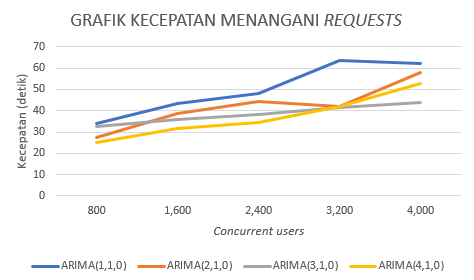
\includegraphics[width=8.7cm,height=4.7cm]{Images/C-5/runningtime.png}
				\caption{Grafik Kecepatan Menangani \textit{Request}}
				\label{grunningtime}
			\end{figure}
            
        \subsubsection{Penggunaan CPU}
        	Dari hasil uji coba penggunaan CPU pada \textit{server master host}, penggunaan CPU berada di bawah 15\%. Penggunaan CPU yang diukur adalah penggunaan CPU yang dilakukan oleh \textit{container} dari aplikasi, tidak termasuk sistem. Jumlah \textit{core} yang dimiliki oleh \textit{processor} di \textit{server master host} adalah 8 buah, yang artinya kurang lebih hanya satu core yang digunakan untuk menangani semua \textit{request}. Hasil pengukuran penggunaan CPU dapat dilihat pada Tabel \ref{penggunaancpu}
            
            \begin{longtable}{|p{0.22\textwidth}|p{0.10\textwidth}|p{0.10\textwidth}|p{0.10\textwidth}|p{0.10\textwidth}|p{0.10\textwidth}|}
        \caption{Penggunaan CPU} \label{penggunaancpu} \\
            \hline
            & \textbf{800} & \textbf{1600} & \textbf{2400} & \textbf{3200} & \textbf{4000} \\ \hline
            \endfirsthead
            \caption[]{Penggunaan CPU} \\
            \hline
            & \textbf{800} & \textbf{1600} & \textbf{2400} & \textbf{3200} & \textbf{4000} \\ \hline
            \endhead
            \endfoot
            \endlastfoot
			
            ARIMA(1,1,0) & 7.1\% & 7.8\% & 9.1\% & 10.5\% & 10.7\% \\ \hline
            ARIMA(2,1,0) & 8.5\% & 9.2\% & 10.1\% & 11.3\% & 10.7\% \\ \hline
            ARIMA(3,1,0) & 8.8\% & 10.2\% & 11.6\% & 12.1\% & 10.3\% \\ \hline
            ARIMA(4,1,0) & 8.0\% & 8.3\% & 10.1\% & 12.9\% & 10.5\% \\ \hline

		\end{longtable}
            
            Dari hasil uji coba, penggunaan prediksi yang berbeda tidak terlalu berpengaruh terhadap penggunaan CPU. Lalu, penggunaan CPU tergolong rendah, yaitu hanya sebesar $\pm 10 \%$ untuk menangani semua \textit{request} yang diberikan. Hasil uji coba performa penggunaan CPU ditunjukkan oleh dalam grafik pada Gambar \ref{gcpuusage}.
            
        	\begin{figure}[H]
				\centering
				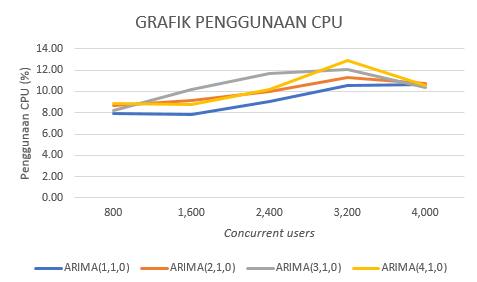
\includegraphics[width=8.7cm,height=4.7cm]{Images/C-5/cpuusage.png}
				\caption{Grafik Penggunaan CPU}
				\label{gcpuusage}
			\end{figure}
            
        \subsubsection{Penggunaan \textit{Memory}}            
            Dari hasil uji coba penggunaan \textit{memory}, semakin banyak \textit{request} yang diterima, semakin banyak \textit{memory} yang diperlukan. Perhitungan penggunaan \textit{memory} adalah rata-rata penggunaan dari masing-masing \textit{container} sebuah aplikasi. Untuk masing-masing \textit{container}, dibatasi penggunaan maksimal \textit{memory} adalah 512 MB. Dari hasil uji coba ini, dapat dilihat pada Tabel \ref{penggunaanmemory} bahwa penggunaan terbesar hanya sebesar 158.71 MB. Artinya jumlah tersebut hanya menggunakan sepertiga dari keseluruhan \textit{memory} yang bisa digunakan.
            \begin{longtable}{|p{0.22\textwidth}|p{0.10\textwidth}|p{0.10\textwidth}|p{0.10\textwidth}|p{0.10\textwidth}|p{0.10\textwidth}|}
        \caption{Penggunaan \textit{Memory}} \label{penggunaanmemory} \\
            \hline
            & \textbf{800} & \textbf{1600} & \textbf{2400} & \textbf{3200} & \textbf{4000} \\ \hline
            \endfirsthead
            \caption[]{Penggunaan \textit{Memory}} \\
            \hline
            & \textbf{800} & \textbf{1600} & \textbf{2400} & \textbf{3200} & \textbf{4000} \\ \hline
            \endhead
            \endfoot
            \endlastfoot
			
           	ARIMA(1,1,0) & 67.91 & 88.97 & 130.79 & 120.14 & 157.73 \\ \hline
            ARIMA(2,1,0) & 65.89 & 97.98 & 123.47 & 156.64 & 158.33 \\ \hline
            ARIMA(3,1,0) & 72.20 & 99.72 & 125.56 & 144.42 & 152.14 \\ \hline
            ARIMA(4,1,0) & 69.60 & 77.34 & 117.39 & 149.76 & 158.71 \\ \hline

		\end{longtable}
            
            Hasil uji coba performa penggunaan \textit{memory} dalam grafik ditunjukkan pada Gambar \ref{gmemoryusage}.
            
        	\begin{figure}[H]
				\centering
				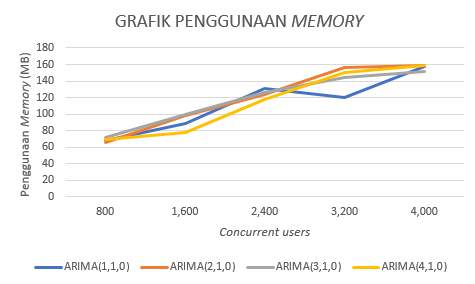
\includegraphics[width=8.7cm,height=4.7cm]{Images/C-5/memoryusage.png}
				\caption{Grafik Penggunaan Memory}
				\label{gmemoryusage}
			\end{figure}
            
        \subsubsection{Keberhasilan \textit{Request}}
        	Pada uji coba ini, dilakukan perhitungan seberapa besar jumlah \textit{request} yang gagal dilakukan. Untuk jumlah \textit{concurrent user} pada tingkat 800 dan 1600, dapat dilihat pada Table \ref{keberhasilanrequest} \textit{error} yang terjadi hampir sama. Prediksi menggunakan ARIMA(4,1,0) berhasil unggul karena menggunakan parameter yang lebih banyak. Namun hal tersebut tidak berlaku untuk ARIMA(3,1,0) karena walaupun parameternya lebih banyak dari ARIMA(2,1,0), tapi hasil prediksinya bisa meleset saat terjadi kondisi dimana koefisien negatif atau koefisien ke dua dikalikan dengan sebuah parameter bukan nol, dan koefisien lain dikalikan dengan parameter nol, maka hasil prediksinya akan negatif, yang mana seharusnya tidak mungkin ada \textit{request} negatif.
            \begin{longtable}{|p{0.22\textwidth}|p{0.10\textwidth}|p{0.10\textwidth}|p{0.10\textwidth}|p{0.10\textwidth}|p{0.10\textwidth}|}
        \caption{\textit{Error Ratio Request}} \label{keberhasilanrequest} \\
            \hline
            & \textbf{800} & \textbf{1600} & \textbf{2400} & \textbf{3200} & \textbf{4000} \\ \hline
            \endfirsthead
            \caption[]{\textit{Error Ratio Request}} \\
            \hline
            & \textbf{800} & \textbf{1600} & \textbf{2400} & \textbf{3200} & \textbf{4000} \\ \hline
            \endhead
            \endfoot
            \endlastfoot
			
            ARIMA(1,1,0) & 5.72\% & 8.96\% & 12.85\% & 12.54\% & 13.38\% \\ \hline
            ARIMA(2,1,0) & 4.31\% & 9.35\% & 10.68\% & 8.11\% & 9.04\% \\ \hline
            ARIMA(3,1,0) & 4.84\% & 10.02\% & 13.22\% & 8.63\% & 12.24\% \\ \hline
            ARIMA(4,1,0) & 4.62\% & 8.41\% & 9.39\% & 7.52\% & 9.21\% \\ \hline
		\end{longtable}
            
    		\begin{figure}[H]
				\centering
				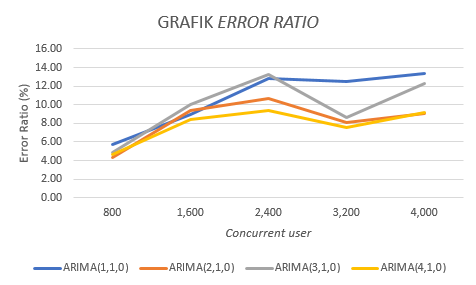
\includegraphics[width=8.7cm,height=4.4cm]{Images/C-5/errorratio.png}
				\caption{Grafik Error Ratio}
				\label{gerrorratio}
			\end{figure}
            Dari uji coba itu, 90\% lebih \textit{request} berhasil ditangani. Hasil uji coba jumlah \textit{request} yang gagal ditunjukkan dengan grafik pada Gambar \ref{gerrorratio}.